\chapter{Verificación simbólica de modelos}

El algoritmo de verificación de modelos con estados explícitos para {\mucalculo} tiene un problema, es muy susceptible a que ocurra una explosión en el tamaño del modelo, especialmente si el grafo de transición de estados se extrae de un sistema concurrente con muchos componentes. \\
\\
\textit{En muchos casos, la “complejidad” del espacio de estados es mucho menor que lo que el número de estados indica. A menudo, los sistemas con un gran número de componentes tienen una estructura regular que sugeriría una regularidad correspondiente en el grafo de estados. En consecuencia, existen representaciones más sofisticadas que explotan esta regularidad. Un buen candidato para tal representación simbólica es el diagrama de decisión binario (BDD)} \cite{Burch:4}.\\ 
\\
En este capítulo se describe un algoritmo de verificación de modelos simbólicos para {\mucalculo} que opera sobre estructuras de Kripke, esta vez representadas no de manera explícita, sino de manera simbólica a través de fórmulas lógicas (que internamente operan como BDDs).

\section{Representación de fórmulas lógicas}

Los árboles binarios de decisión ordenados (OBDDs) son formas canónicas de representación de fórmulas lógicas. Son considerablemente más compactos que las formas normales tradicionales como la forma normal conjuntiva y la forma normal disyuntiva, y existen algoritmos para manipularlos eficientemente. Por esto, los OBDDs se han utilizado para una amplia variedad de aplicaciones en el diseño asistido por computadoras, incluyendo simulación simbólica, verificación de lógica combinatoria y verificación de sistemas concurrentes con estados finitos \cite{Clarke:1}. Las definiciones que aparecen en esta sección se extraen de \cite{Clarke:1}.

\noindent Para entender la necesidad de usar OBDDs, consideremos primero los árboles binarios de decisión. Un árbol binario de decisión es un árbol dirigido con raíz que consiste en vértices terminales y no terminales. Cada vértice no terminal $v$ esta etiquetado por una variable $var(v)$ y tiene dos hijos: $izq(v)$ corresponde al caso en que $v$ tenga el valor 0 y $der(v)$ en caso contrario. Cada vértice terminal esta etiquetado por una constante $valor(v)$ la cual es 0 o 1. Un árbol binario de decisión para la fórmula $f(a,b,c) = (a \land b) \lor (a \land c)$ es mostrado en la figura \ref{fig:bdt1}. Uno puede decidir si una asignación particular a las variables hace verdadera la fórmula o no al atravesar el árbol desde la raíz hasta un vértice terminal. Por ejemplo, la asignación $\{ a \gets 1, b \gets 0, c \gets 0\}$ lleva al vértice terminal 0, por lo tanto la fórmula es falsa para esta asignación.

\begin{figure}[h!]
  \centering
  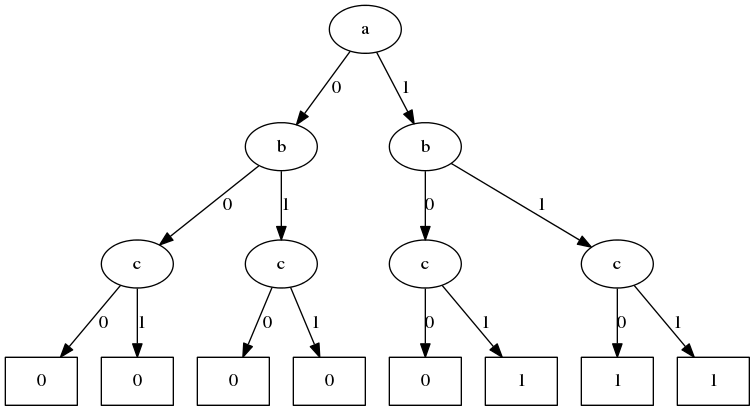
\includegraphics[width=1\textwidth]{Figures/BDT.png}
  \caption{Árbol binario de decisión para este ejemplo.}
  \label{fig:bdt1}
\end{figure}

\noindent Los árboles binarios de decisión no proveen una representación muy concisa para las funciones lógicas. De hecho, tienen el mismo tamaño que las tablas de verdad. Afortunadamente, es común que haya mucha redundancia en tales árboles. Por ejemplo, en la figura \ref{fig:bdt1} todos los caminos donde a tiene el valor 0 llevan al nodo terminal 0, por lo tanto no seria necesario analizar los valores de $b$ y $c$ en esta rama. Esto lleva a pensar que hay formas de reducir el tamaño del árbol unificando subárboles isomorfos. Esto da como resultado un grafo acíclico dirigido (DAG) llamado diagrama binario de decisión (BDD). Mas precisamente, un BDD es un grafo con raíz, dirigido y acíclico con dos tipos de vértices, vértices terminales y no terminales. Estos tienen el mismo significado que en el caso de los árboles. Cada BDD $B$ con raiz $v$ determina una función lógica $f_{v}(x_{1},...,x_{n})$ de la siguiente manera \cite{Clarke:1}:\\
\\
1. Si $v$ es un vértice terminal:
  (a) Si $valor(v) = 1$ entonces $f_{v}(x_{1},...,x_{n}) = 1$.
  (b) Si $valor(v) = 0$ entonces $f_{v}(x_{1},...,x_{n}) = 0$.\\
\\
2. Si $v$ es un vértice no terminal con $var(v) = x_{i}$ entonces $f_{v}$ es la función 
\[f_{v}(x_{1},...,x_{n}) = (\neg x_{i} \land f_{izq(v)}(x_{1},...,x_{n})) \lor (x_{i} \land f_{der(v)}(x_{1},...,x_{n}))\]\\
\noindent Bryant \cite{Bryant:8} demostró como obtener una representación canónica para funciones lógicas al poner dos restricciones sobre los BDDs. Primero, las variables deberían aparecer en el mismo orden a lo largo de cada camino desde la raiz a un terminal. Segundo, no debería haber subárboles isomórficos o vértices redundantes en el diagrama. El primer requisito se logra al imponer un ordenamiento total $<$ sobre las variables que etiquetan los vértices en el BDD y requiriendo eso para cada vértice $u$ en el diagrama, si $u$ tiene un sucesor no terminal, entonces $var(u) < var(v)$. El segundo requisito se logra al aplicar repetidamente tres reglas de transformación que no alteran la función representada por el diagrama, \\
\\
- Eliminar terminales duplicados: Dejar solo un terminal para cada valor y redirigir todos los arcos a los eliminados hacia este.\\
\\
- Eliminar no terminales duplicados: Si dos no terminales $u$ y $v$ tienen $var(u) = var(v), izq(u) = izq(v) y der(u) = der(v)$, entonces eliminar $u$ o $v$ y redirigir todos los arcos que iban al vértice eliminado hacia el otro.\\
\\
- Eliminar tests redundantes: Si el no terminal $v$ tiene $izq(v) = der(v)$, entonces eliminar $v$ y redirigir todos los arcos a $izq(v)$.\\
\\
Empezando por un BDD satisfaciendo la propiedad de ordenamiento, la forma canónica se obtiene aplicando las reglas de transformación hasta que el tamaño del diagrama no pueda ser reducido. Al resultado lo vamos a llamar OBDD.\\
\\
Hay que destacar que el tamaño del OBDD depende fuertemente del ordenamiento de las variables. Esto se puede ver en las figuras \ref{fig:gord1} y \ref{fig:bord1}
\begin{figure}[H]
  \centering
  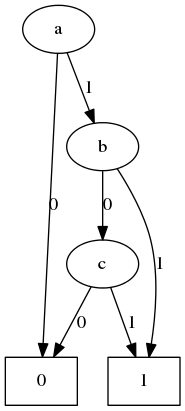
\includegraphics[width=0.2\textwidth]{Figures/goodorder.png}
  \caption{OBDD con ordenamiento a < b < c para el ejemplo dado.}
  \label{fig:gord1}
\end{figure}
\begin{figure}[H]
  \centering
  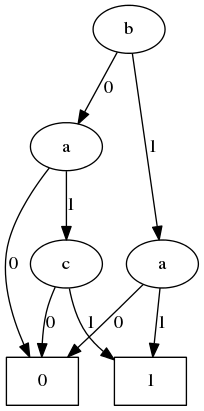
\includegraphics[width=0.2\textwidth]{Figures/badorder.png}
  \caption{OBDD con ordenamiento b < a < c para el ejemplo dado.}
  \label{fig:bord1}
\end{figure}

\section{Representación de estructuras de Kripke}

Para ilustrar como los OBDDs pueden ser usados para representar concisamente una estructura de Kripke, consideremos la estructura de dos estados mostrada en la figura \ref{fig:kripke2} donde $L(s_{1}) = \{x,y\}$ y $L(s_{2}) = \{x,y,z\}$. En este caso hay tres variables de estado, $x$, $y$, y $z$. Introducimos tres variables más, $x'$, $y'$ y $z'$, para representar el estado sucesor. Asi, representaremos la transición de $s_{1}$ a $s_{2}$ como la conjunción:

$(x \land y \land \neg z \land x' \land y' \land z')$\\
\\
La fórmula lógica para todo el sistema de transiciones esta dada por:

$(x \land y \land \neg z \land x' \land y' \land z') \lor (x \land y \land \neg z \land x' \land y' \land \neg z') \lor (x \land y \land z \land x' \land y' \land \neg z') \lor (x \land y \land z \land x' \land y' \land z')$ 
\begin{figure}[H]
  \centering
  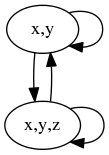
\includegraphics[width=0.2\textwidth]{Figures/kripke2.png}
  \caption{Estructura de Kripke con dos estados.}
  \label{fig:kripke2}
\end{figure}

\noindent En la fórmula hay cuatro disyuntos porque la estructura de Kripke tiene cuatro transiciones. Esta fórmula se convierte ahora en OBDD para obtener una representación concisa de la relación de transición.\\
\\
En muchos casos, construir una representación explicita de la estructura de Kripke $M$ y luego codificarla como se vió anteriormente no es factible porque la estructura es demasiado grande, incluso si la representación simbólica termina siendo concisa. Por lo tanto, en la práctica construimos los OBDDs directamente desde una descripción de alto nivel del sistema. En el próximo capitulo, cuando introduzcamos el lenguaje de modelado de sistemas utilizado en este trabajo, veremos como se realiza esta transformación.

\section{Algoritmo de verificación simbólica de modelos}

En la sección anterior vimos como codificar una estructura de Kripke como un OBDD, ahora mostraremos una adaptación del algoritmo de verificación con estados explícitos, ahora con una representación simbólica del modelo en forma de OBDD. En este caso transformaremos las fórmulas del {\mucalculo} de la siguiente manera\cite{Clarke:1}: \\
\\
- Los valores Falso y Verdadero están representados por OBDD-FALSE y OBDD-TRUE que son constantes(hojas).\\
\\
- Cada proposición atómica $p$ tiene un OBDD asociado con el mismo. Lo denotaremos como $OBDD_{p}(x)$, donde x es un estado del sistema, este OBDD cumple la propiedad de que $x$ satisface $OBDD_{p}$ si y solo si $x \in L(p)$. \\
\\
- El sistema de transiciones tiene un diagrama ordenado de decisión $OBDD_{m}(x,x')$ asociado al mismo. Un par $(x,x') \in S \times S$ satisface $OBDD_{m}$ si y solo si $(x,x') \in T$ \\
\\
Asumamos que tenemos una fórmula $f$ de {\mucalculo} con las variables relacionales libres $Q_{1},...,Q_{k}$. La función $assoc[Q_{i}]$ asigna a cada variable relacional el OBDD correspondiente al conjunto de estados asociados a esa variable. La notación $assoc(Q \gets B_{Q})$ significa que a $Q$ se le da el valor $B_{Q}$, se puede ver a $assoc$ como un ambiente de OBDDs. A continuación se da el procedimiento $B$ que, a partir de una fórmula $f$ y una función $assoc$, retorna el OBDD correspondiente a la semántica de $f$.

\begin{align*}
 B(p,assoc)\ &=\ OBDD_{p}(x) \\
 B(Q_{i},assoc)\ &=\ assoc[Q_{i}] \\
 B(\neg f,assoc)\ &=\ \neg B(f,assoc) \\
 B(f \land g,assoc)\ &=\ B(f,assoc) \land B(g,assoc) \\
 B(f \lor g,assoc)\ &=\ B(f,assoc) \lor B(g,assoc) \\
 B(\Diamond f,assoc)\ &=\ \exists x' : OBDD_{m}(x,x') \land B(f,assoc)(x') \\
 B(\Box f,assoc)\ &=\ B(\neg \Diamond \neg f, assoc) \\
 B(\mu Q. f, assoc) &= FIX(f,assoc,OBDD-FALSE) \\
 B(\nu Q. f, assoc) &= FIX(f,assoc,OBDD-TRUE) \\
\end{align*}

\noindent Donde $B(f,assoc)(x')$ reemplaza cada aparición de $x$ por $x'$, y FIX es la siguiente función:
\begin{figure}[H]
  \centering
  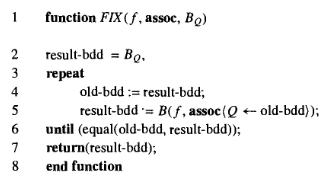
\includegraphics[width=0.7\textwidth]{Figures/fix.png}
  \caption{Pseudocódigo de la función FIX \cite{Clarke:1}.}
  \label{fig:fix}
\end{figure}

\noindent Las operaciones lógicas que ocurren del lado derecho de las ecuaciones son operaciones de BDDs. El significado de la cuantificación existencial de una variable lógica está dada por la siguiente ecuación \cite{Andersen:7} :

\[ \exists x . t = t[0/x] \lor t[1/x]\] 

Donde $t[v/x]$ es t pero donde x toma el valor v.

\subsection{Complejidad}

Un interrogante importante en cuanto a la verificación de modelos para {\mucalculo} es su complejidad. Los algoritmos más eficientes conocidos son exponenciales en cuanto al tamaño de la fórmula. Existe la conjetura\cite{Clarke:1} de que no hay un algoritmo polinomial para el problema de la verificación de modelos para {\mucalculo}. Es posible demostrar que el problema esta en $NP \cap co-NP$. Si el problema fuera NP-completo, entonces NP seria igual a co-NP, lo cuál se cree que no es cierto.
